\documentclass{article}
\usepackage[utf8]{inputenc}
\usepackage{amsmath, amssymb}
\usepackage{mathtools}
\usepackage{a4wide}
\usepackage{appendix}
\usepackage{listings}
\usepackage{float}
\usepackage{subcaption}
\usepackage{hyperref}

\title{Optic flow}
\author{Hugo (s214734) \and Mikael H. Hoffmann (s214753) \and Christian Valentin Kjær (s211469) \and Jacob Tuxen (s194572)}
\date{\today}

\begin{document}

\maketitle

\section{Introduction (problem and background)}
Optical flow is a method to determine object motion in video, based on the relative displacement of pixels
through time in the video. To obtain such a motion prediction, a few strong assumptions are made about the subject video, including:
\begin{itemize}
    \item There has been only a small displacement through time
    \item There are no changes in the lighting
    \item Pixel intensity alone is enough to determine movement in the video
\end{itemize}
These assumptions are necessary for applying a mathematical model to the problem of optic flow.

\section{Data and experiments - Jacob} 
\subsection{Data and Materials}
All the data used in this project regarding optical flow, are videos. All the videos used have dimensions \{frames, width, height, depth\}. The depth refers to the layers of color, we captured our videos in color, this means there were 3 layers, RGB. The frames describe how many pictures the video contained, and the width and height correspond to the pixels in the horizontal and vertical direction. 1 Video from the data pool where an animated ball, the others were videos we captured.
\\\\
The materials used were:
\begin{itemize}
    \item Smartphone for video capturing
    \item PC for processing video in python
    \item Movable objects to capture
\end{itemize}
\subsection{Experiments and Physical Method}
The general experiments all follow the same procedure. We wanted to capture a video, and then process the optical flow using the mathematical model described below to detect movement in the video.
As we have mentioned before optical flow does have some disadvantages, namely no change in lightning and only smaller displacements through time. We sought to make a video with movement that was detectable, and had the same environmental influences throughout the video. This means no changing lighting and a steady camera.
\\
Furthermore we also wanted to capture a video where we know that optical flow would not work. This was done in order to see the unreliability of our model. The video we tried to do this was with a shadow moving over a surface. And thoughts were that the optical flow would detect movement even though, no movement was present but only change in lightning.


\section{Mathematical model and image processing methodology}
We start by considering the point $\boldsymbol{p} = [p_x, p_y, p_t]$ and we want to find the vector $\boldsymbol{u} = [x, y, 1]$ which represents the movement of the above mentioned pixel in \emph{one} time frame. If $\boldsymbol{V(p)}$ represents the pixel value then $\boldsymbol{u}$ satisfies 

\begin{equation}\label{eq:initial-equation}
    \boldsymbol{V(p + u)} = \boldsymbol{V(p)}.
\end{equation}

This also means that we are assuming constant brightness.

If the displacement is small then it is possible to  approximate the movement with a first order Taylor expansion

\begin{equation}
    \boldsymbol{V(p + u)} = \boldsymbol{V(p)} + \begin{bmatrix}
        \boldsymbol{V}_x(\boldsymbol{p}) & \boldsymbol{V}_y(\boldsymbol{p}) & \boldsymbol{V}_t(\boldsymbol{p})
    \end{bmatrix} \boldsymbol{u}.
\end{equation}
Where $[\boldsymbol{V}_x(\boldsymbol{p}),\boldsymbol{V}_y(\boldsymbol{p}),\boldsymbol{V}_t(\boldsymbol{p})]$ are the value of the gradient in the $x,y,t$ directions respectively. Inserting this in equation \ref{eq:initial-equation} yields

\begin{equation}
    \begin{split}
        \boldsymbol{V(p)} + \begin{bmatrix}
        \boldsymbol{V}_x(\boldsymbol{p}) & \boldsymbol{V}_y(\boldsymbol{p}) & \boldsymbol{V}_t(\boldsymbol{p})
        \end{bmatrix} \boldsymbol{u} - \boldsymbol{V(p)} &= \boldsymbol{V}_x(\boldsymbol{p}) x + \boldsymbol{V}_y(\boldsymbol{p}) y + \boldsymbol{V}_t(\boldsymbol{p}) \cdot 1 \\
        &= 0,
    \end{split}
\end{equation}

and rearranging gives

\begin{equation}\label{eq:final-model}
    \boldsymbol{V}_x(\boldsymbol{p}) x + \boldsymbol{V}_y(\boldsymbol{p}) y = -\boldsymbol{V}_t(\boldsymbol{p}).
\end{equation}

\subsection{Lucas Kanade solution}
The equation in (\ref{eq:final-model}) is an under determined since there is one equation with 2 unknowns, it is not possible to determine a solution for $x$ and $y$. Considering a point $\textbf{p}=[p_x,p_y,p_t]$, Lucas Kanade's method suggest to assume that all pixels within a small neighborhood of $\textbf{p}$ have the same movement. This assumptions implies that (\ref{eq:final-model}) can be expanded by solving for all points within the neighborhood of \textbf{p}, which yields the following system.
\begin{equation}\label{LK}
    \begin{bmatrix}
        \vdots & \vdots \\
        \boldsymbol{V}_x(\boldsymbol{p}_i) & \boldsymbol{V}_y(\boldsymbol{p}_i) \\
        \vdots & \vdots
    \end{bmatrix} \begin{bmatrix}
        x \\ y
    \end{bmatrix}
    = - \begin{bmatrix}
        \vdots \\ \boldsymbol{V}_t(\boldsymbol{p}_i) \\ \vdots
    \end{bmatrix}.
\end{equation}
The system in (\ref{LK}) is an over determined linear system with $n$ equations and 2 unknowns, where $n$ is the number of pixels in the neighbourhood around \textbf{p}. Such a system can be solved using least squares.

To conclude the optical flow in each pixel is obtained by assuming that each pixels within a small neighbourhood of each share the same movement. 

\subsection{Image processing methodology}
In image processing an image is expressed as a single matrix for gray scale images and 3 matrices for RGB images. This representation allows us to manipulate the images using linear algebra and other areas of mathematics involving matrices. In the given problem for optical flows the calculations rely on image gradients, Taylor expansions and linear least squares. 

\section{Visualise results - Mikael}
When running the code with the supplied test video and our custom video we got the following

\begin{figure}[H]
    \begin{subfigure}{.5\textwidth}
        \centering
        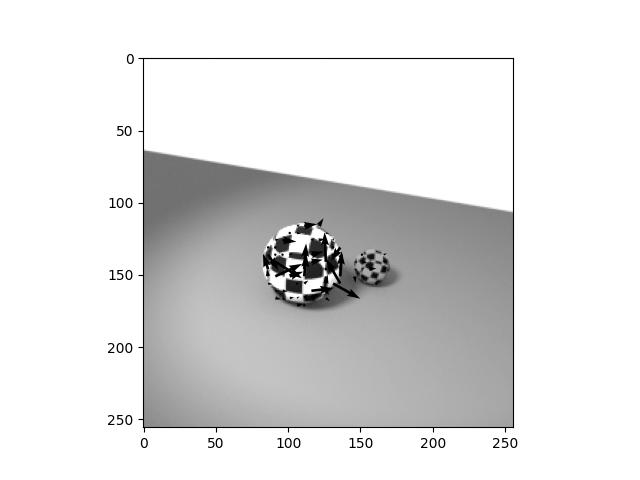
\includegraphics[scale=0.4]{code/toyProblem_F22_vectorField/48.jpg}
        \caption{The 48th frame with arrows indicating the size and movement of selected pixels.}
        \label{fig:moving-ball}
    \end{subfigure}%
    \begin{subfigure}{.5\textwidth}
        \centering
        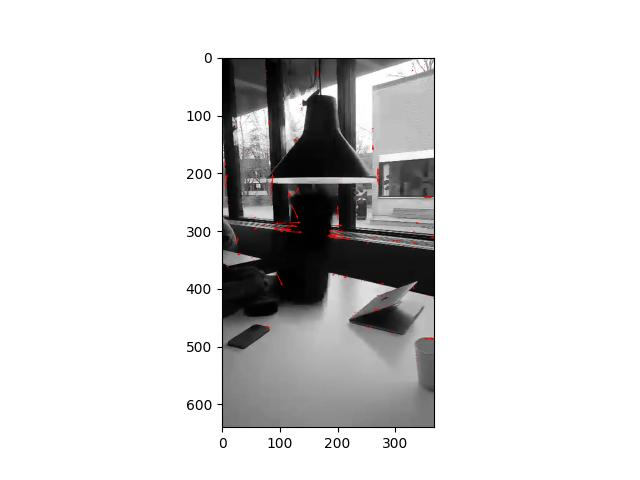
\includegraphics[scale=0.4]{code/vanteImages_vectorField/32.jpg}
        \caption{Placeholder!}
        \label{fig:custom-video}
    \end{subfigure}
\end{figure}

In both cases we see that \dots

\section{Discuss results - }

\section{Conclude}
A complete python implementation of the Lucas Kanade solution and some of its variations, to the optical flow problem, is created and applied to various optical flow problems. These are used to illustrate both strengths and weeknesses of the Lucas Kanade optical flow solution - see figures ???, ??? and ???.
% By applying the Lucas Kanade method to optical flow, we have shown the dependency of optical flow to lighting conditions. Moreover 





\section{Exercise (5)}
Define $A$ as per equation (2) in the handout:
\begin{equation}
    A = \begin{bmatrix}
    \vdots & \vdots \\
    V_{x}(p_i) & V_{y}(p_i) \\
    \vdots & \vdots
    \end{bmatrix}
\end{equation}
Then the normal equation to $Ax = b$ will have the system matrix (where $N$ denotes the considered neighborhood):
\begin{equation}
    A^\intercal A = \begin{bmatrix}
        \sum_{i \in N} V_{x}(p_i)^{2} & \sum_{i \in N} V_{x}(p_i)V_{y}(p_i) \\
        \sum_{i \in N} V_{x}(p_i)V_{y}(p_i) & \sum_{i \in N} V_{y}(p_i)^{2}
    \end{bmatrix}
\end{equation}
Which we could also get by passing a filter of all ones over $N$ in $V_x$ and $V_y$.

\newpage
\appendix
\section{Code}
To view the code in a proper folder structure, refer to our github: \url{https://github.com/ElMiho/02526-mathematical-modeling-project-1}



\subsection{Exercise 1}
\lstinputlisting[language=Python,breaklines=true]{code/exercise_1.py}

\subsection{Exercise 2}
\lstinputlisting[language=Python,breaklines=true]{code/exercise_2.py}

\subsection{Exercise 3}
\lstinputlisting[language=Python,breaklines=true]{code/exercise_3.py}

\subsection{Various functions}
\lstinputlisting[language=Python,breaklines=true]{code/functions.py}

\subsection{Video plotter}
\lstinputlisting[language=Python,breaklines=true]{code/video_plotter.py}

\subsection{Main}
\lstinputlisting[language=Python,breaklines=true]{code/main.py}


\end{document}
